\documentclass{beamer}
\usepackage[utf8]{inputenc}
\usepackage{hyperref}
\usepackage{multicol}
\usepackage{hyperref}
\usepackage{amsmath}
\usepackage[english]{babel}
\usepackage{algorithm}
\usepackage[noend]{algpseudocode}

\inputencoding{utf8}

\mode<presentation> {
    \usetheme{Madrid}
}

\usepackage{graphicx}
\usepackage{booktabs}

\title[Codiciosos]{Analisis Aromatizado}
\author{Ernesto Rodriguez - Juan Roberto Alvaro Saravia}
\institute{
    Universidad Francisco Marroquin \\
    \medskip \textit{ernestorodriguez@ufm.edu - juanalvarado@ufm.edu}
}

\date[\today]{}

\begin{document}

\begin{frame}
\titlepage
\end{frame}

\begin{frame}
\frametitle{Ejemplo: Pila}
\begin{itemize}
    \item{Se tienen dos operaciones: $\mathtt{Push}$ y $\mathtt{Pop}$}
    \item{Cada operaci\'on toma un tiempo constante $c$}
    \item{Por lo tanto una secuencia de $N$ operaciones toma $cN$}
    \item{Por lo tanto el promedio es $\frac{cN}{N}=c$}
\end{itemize}
\end{frame}

\begin{frame}
\frametitle{Operaci\'on Multipop}
\begin{itemize}
    \item{Operaci\'on que ejecuta pop $k$ veces}
    \item{Si $k>n$, solo se ejecuta $n$ veces}
    \item{Tiempo de ejecuci\'on es $\mathcal{O}(n)$}
\end{itemize}
\begin{algorithm}[H]
    \caption{Multipop}
    \begin{algorithmic}[1]
    \Procedure{Multipop}{$S,k$}
    \While{$\mathtt{len}(S)>0$ {\bf and} $k>0$}
        \State{$\mathtt{Pop}(S)$}
        \State{$k\gets k-1$}
    \EndWhile
    \EndProcedure
    \end{algorithmic}
\end{algorithm}
\end{frame}

\begin{frame}
\frametitle{Tiempo Promedio}
\begin{itemize}
    \item{Se considera una secuencia de $N$ operaciones,
    las cuales pueden ser $\mathtt{Push}$, $\mathtt{Pop}$
    y $\mathtt{Multipop}$
    \begin{itemize}
        \item{¿Cual es el tiempo de ejecuci\'on de $N$ operaciones?}
        \item{¿Que pasa si la pila esta vacia?}
    \end{itemize}
    }
\end{itemize}
\end{frame}

\begin{frame}
    \frametitle{Analisis Aromatizado}
    \begin{itemize}
        \item{Consiste en calcular el tiempo promedio que tomaria una secuencia de operaciones.}
        \item{Difiere de la complejidad promedio:
        \begin{itemize}
            \item{Es el tiempo promedio que toma cada operaci\'on en una secuencia de
            operaciones}
            \item{Siempre se considera el peor caso del input}
            \item{Ie. la cantidad de ciclos es la peor, pero el tiempo que toma
            cada ciclo se promedia.}
        \end{itemize}
        }
        \item{Al final, en vez de tener $n$ operaciones de costo diferente,
        se obtiene el promedio repetido $n$ veces.}
        \item{El ejemplo anterior se llama \emph{Analisis Acumulado}}
        \item{Applicaciones: Scheduling de procesos}
    \end{itemize}
    \end{frame}
    
\begin{frame}
\frametitle{Analisis Acumulado}
\begin{itemize}
    \item{Se considera una secuencia de $n$ operaciones}
    \item{Cada operaci\'on tiene un costo $T(n)$}
    \item{Por eso mismo, el costo promedio de cada operaci\'on
    seria $T(n)/n$}
\end{itemize}
\end{frame}

\begin{frame}
\frametitle{Ejemplo: Contador Binario}
\begin{itemize}
    \item{Se tiene un numero $c$ de $k$ bits.}
    \item{Cada bit se almacena en un arreglo de tama\~no $k$.}
    \item{En la posici\'on $0$ del arreglo se encuentra el bit de
    menor orden}
    \item{En la posici\'on $k-1$ del arreglo se encuentra el bit de
    mayor orden}
    \item{Por eso mismo $c=\sum_{i=0}^{k-1}A[i]*2^i$}
\end{itemize}
\end{frame}

\begin{frame}
\frametitle{Incrementando el Contador}

\begin{algorithm}[H]
    \caption{Incrementar}
    \begin{algorithmic}[1]
    \Procedure{Incrementar}{$A$}
    \State{$i\gets 0$}
    \While{$i<\mathtt{len}(A)$ {\bf and} $A[i]\equiv 1$}
        \State{$A[i]\gets 0$}
        \State{$i\gets i+1$}
    \EndWhile
    \If{$i<\mathtt{len}(A)$}
        \State{$A[i]\gets 1$}
    \EndIf
    \EndProcedure
    \end{algorithmic}
\end{algorithm}

\end{frame}

\begin{frame}
\frametitle{Analisis Asintotico}
\begin{itemize}
    \item{Cada ejecuci\'on de $\mathtt{Incrementar}$ toma $\mathcal{O}(k)$
    operaciones}
    \item{Se ejecuta $\mathtt{Incrementar}$ $n$ veces.}
    \item{El tiempo de ejecuci\'on es $\mathcal{O}(nk)$}
\end{itemize}
¿Podemos ser mas precisios?
\end{frame}

\begin{frame}
\frametitle{Incrementando el Contador}

\begin{center}
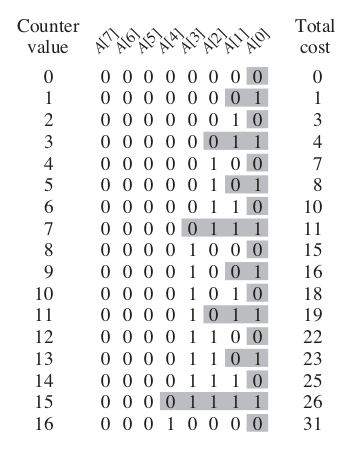
\includegraphics[width=6cm]{inc.png}
\end{center}
    
\end{frame}

\begin{frame}
\frametitle{Analisis Asintotico}
\begin{itemize}
    \item{El primer bit se debe cambiar en cada operaci\'on}
    \item{Sin embargo, el segundo bit se cambia cada dos operaciones}
    \item{El cuarto bit se cambia cada cuatro operaciones}
    \item{etc...}
\end{itemize}
\end{frame}

\end{document}